\documentclass[conference]{IEEEtran}
\usepackage{cite}
\usepackage{amsmath,amssymb,amsfonts}
\usepackage{algorithmic}
\usepackage{graphicx}
\usepackage{textcomp}
\usepackage{xcolor}
\graphicspath{{figures/}}

\begin{document}

\title{Trade-off Analysis between Accuracy and Computational Efficiency in Sarcasm Detection Using DistilBERT and RoBERTa}

\author{\IEEEauthorblockN{Falah Razan Hibrizi}
\IEEEauthorblockA{\textit{School of Computing} \\
\textit{Telkom University}\\
Bandung, Indonesia \\
email address}
\and
\IEEEauthorblockN{Supervisor Name}
\IEEEauthorblockA{\textit{School of Computing} \\
\textit{Telkom University}\\
Bandung, Indonesia \\
email address}
}


\maketitle

\begin{abstract}
Sarcasm often expresses the opposite of its literal meaning, which causes sentiment analysis systems to misread it. This study examines the trade-off between performance and computational efficiency of RoBERTa and DistilBERT on 1,000,864 comment and parent comment pairs from the Self-Annotated Reddit Corpus (SARC). The comparison covers three input configurations, namely comment only, early fusion, and late fusion, as well as partial layer freezing. The final configurations were selected on validation data and locked before any test score was computed. Each configuration was run with three seeds and evaluated with the paired t-test, the Wilcoxon signed-rank test, and the Friedman test with Holm correction. The highest macro-F1 of 79.62\% was obtained by RoBERTa with early fusion, and RoBERTa outperformed DistilBERT by 1.65--2.07 points. Nevertheless, DistilBERT reached 97--98\% of the RoBERTa macro-F1 with about half of the training time, latency, and GPU memory. The parent comment raised macro-F1 by 0.69--1.10 points, mainly on ambiguous comments. For RoBERTa, early fusion was more accurate and far cheaper than late fusion. Freezing 6 of the 12 RoBERTa layers reduced macro-F1 by only 0.24 points and cut training time by about 45\%, but inference latency did not decrease. RoBERTa is preferable when accuracy is the priority, whereas DistilBERT is more suitable under latency and memory constraints.
\end{abstract}

\begin{IEEEkeywords}
computational efficiency, DistilBERT, layer freezing, parent comment, RoBERTa, sarcasm detection
\end{IEEEkeywords}

\section{Introduction}
In sarcasm, the speaker says something opposite to what is actually meant, for example using a compliment to mock. Such sentences are difficult for sentiment analysis systems because words that look positive carry a negative intent \cite{prakash2025sarcasm}. As a result, public opinion monitoring and content moderation may produce wrong outputs, including in cyberbullying detection on social media \cite{dhumpati2025sarcasm}, \cite{grover2026emoji}.

Written text offers no tone of voice or facial expression as a cue \cite{jimenez2026bert}. On Reddit, the sarcastic nature of a reply often becomes clear only after the reader knows the comment being replied to, called the parent comment. The Self-Annotated Reddit Corpus (SARC) \cite{khodak2018sarc} provides a very large number of parent comment and reply pairs. Other context, such as user information and forum topic, also helps models on SARC \cite{hao2023enhanced}, and feeding the parent comment into a transformer model has been reported to improve performance \cite{ataeii2020transformers}, \cite{dubey2025unpacking}.

RoBERTa \cite{liu2019roberta} is a refinement of BERT with an improved pretraining procedure. It generally achieves high accuracy, but its memory and computation requirements are large, while computing resources are limited \cite{treviso2023efficient}. DistilBERT \cite{sanh2019distilbert} is obtained through knowledge distillation, so it has half the layers and faster inference. Studies comparing BERT variants for sarcasm detection show that performance depends strongly on the choice of model and training settings \cite{jimenez2026bert}, \cite{ullah2026advanced}.

Dubey et al.\ compared RoBERTa and DistilBERT, including on SARC, and reported that DistilBERT trained about 1.74 times faster with competitive performance \cite{dubey2025unpacking}, \cite{dubey2026efficient}. However, both models were combined with BART context summaries and metadata embeddings, the experiments used only a subset of 7,370 samples \cite{dubey2025unpacking}, and the preprocessing removed capitalization and punctuation, which can signal sarcasm \cite{dubey2026efficient}. The difference between the two models in \cite{dubey2026efficient} was also not significant ($p = 0.064$). Zhang et al.\ \cite{zhang2025enhancing} used SARC at a larger scale but did not separate test data from validation data. Moreover, the way the parent comment is fed into the model and layer freezing have rarely been discussed together with their computational cost.

Therefore, this study compares the performance and computational efficiency of RoBERTa and DistilBERT on approximately one million SARC comment pairs without additional components, and analyzes their trade-off through the following three research questions.
\begin{enumerate}
\item Does the number of frozen layers affect sarcasm classification performance?
\item Does using the parent comment as input affect sarcasm classification performance?
\item Which fusion strategy yields the best sarcasm classification performance?
\end{enumerate}
Each question is answered for both models while taking into account training time, inference latency, GPU memory, and number of parameters. The contributions of this study are (i) a comparison with light preprocessing, configurations locked before the test data were opened, three seeds, and statistical tests with Holm correction; (ii) measurements of computational cost for three inputs and several levels of layer freezing; and (iii) an analysis of the types of comments that benefit most from the parent.

\section{Methodology}

\subsection{Dataset and Preprocessing}
\label{sec:data}
This study uses the balanced version of SARC \cite{khodak2018sarc} from Kaggle, the same as in \cite{dubey2026efficient}, \cite{zhang2025enhancing}, which contains 1,010,826 comment and parent comment pairs. The labels come from the ``/s'' marker added by the comment authors, and this marker was removed from the text \cite{khodak2018sarc}.

Unlike \cite{dubey2026efficient}, \cite{zhang2025enhancing}, which lowercased the text, removed punctuation, and applied lemmatization, preprocessing here was kept light because capitalization, punctuation, and emoticons such as ``;)'' may indicate sarcasm. Cleaning consisted only of decoding HTML entities, replacing Markdown links with their text, removing URLs and HTML tags, and normalizing whitespace, so only 2,942 comments (0.29\%) were changed.

The filtering steps are shown in Table~\ref{tab:data}. Duplicates and conflicting labels were detected with a normalized key (lowercase, without punctuation), but the model still received the original text. The last step removed residual ``/s'' artifacts in the form of sentence fragments such as ``You forgot the'', matched with a pattern of at most eight words. Of the 8,599 matching rows, 8,580 were labeled sarcastic, so all of them were removed to prevent the model from learning this shortcut. The result is 1,000,864 pairs with a sarcastic proportion of 49.59\%.

\begin{table}[t]
\caption{Row Filtering and Data Split}
\label{tab:data}
\centering
\begin{tabular}{lrr}
\hline
Filtering step & Removed & Remaining \\
\hline
Raw data & -- & 1,010,826 \\
Empty comment & 55 & 1,010,771 \\
Empty after cleaning & 9 & 1,010,762 \\
Conflicting labels & 142 & 1,010,620 \\
Duplicate pairs & 1,157 & 1,009,463 \\
``/s'' fragments & 8,599 & 1,000,864 \\
\hline
Split & Pairs & Sarcastic (\%) \\
\hline
Training & 799,459 & 49.66 \\
Validation & 100,276 & 49.38 \\
Test & 101,129 & 49.27 \\
\hline
\end{tabular}
\end{table}

The data were split with seed 42 by comment group rather than by row, because short replies such as ``Source?'' appear hundreds of times. The result is close to an 80/10/10 ratio, with no comment or pair appearing in more than one split.

\subsection{Models and Input Configurations}
RoBERTa-base \cite{liu2019roberta} has 12 layers, a hidden size of 768, and 124.6 million parameters, whereas DistilBERT \cite{sanh2019distilbert} has six layers and 65.8 million parameters. The cased version of DistilBERT was chosen so that both models can distinguish capitalization. Three input configurations were compared.

\textit{Comment only.} The model receives only the reply text as the baseline.

\textit{Early fusion.} The parent and comment are combined with the tokenizer's sentence-pair format, with the parent first, similar to \cite{ataeii2020transformers}, so every comment token can attend to all parent tokens from the first layer. The input is limited to 256 tokens by truncating the end of the parent, which happens for 0.85\% of the RoBERTa training pairs and 0.99\% for DistilBERT. Only 52--54 comments exceed 256 tokens (less than 0.01\%).

\textit{Late fusion.} The parent and comment are encoded separately with the same encoder. The final hidden states at the first token of the comment ($h_x$) and of the parent ($h_y$) are combined into
\begin{equation}
u = [\,h_x;\; h_y;\; |h_x - h_y|;\; h_x \odot h_y\,],
\label{eq:fusion}
\end{equation}
where $[\cdot\,;\cdot]$ denotes concatenation and $\odot$ element-wise multiplication. The vector $u$ is passed to the default classification head of the model with a four times larger input size. Consequently, the encoder runs twice per example and comment tokens cannot attend directly to parent tokens.

\subsection{Layer Freezing}
Layer freezing is a form of selective fine-tuning because only a subset of the parameters is trained \cite{han2024peft}, and it can save GPU memory with only a small loss in accuracy \cite{ardakani2024slimfit}. The embedding layer and a number of the lowest layers were frozen in early fusion, namely 0, 6, 9, and 12 of the 12 RoBERTa layers and 0, 3, and 6 of the 6 DistilBERT layers. Partially frozen models used the best learning rate from full fine-tuning with three seeds. For fully frozen models, learning rates of $10^{-4}$ and $10^{-3}$ were tried with seed 42 and the better one on validation was selected. Freezing reduces only the training cost because all layers are still executed during inference.

\subsection{Experimental Setup}
The training settings are summarized in Table~\ref{tab:setup}. Biases and LayerNorm parameters were excluded from weight decay, and each batch was padded only to its longest sequence. The learning rate was selected through a grid search because RoBERTa is sensitive to training settings \cite{jimenez2026bert}, and the grid includes the values used in \cite{dubey2026efficient}, \cite{ullah2026advanced}.

\begin{table}[t]
\caption{Training Settings}
\label{tab:setup}
\centering
\begin{tabular}{ll}
\hline
Setting & Value \\
\hline
Maximum input length & 256 tokens \\
Batch size & 32 (evaluation: 128) \\
Epochs & max. 3, best by validation macro-F1 \\
Optimizer & AdamW, weight decay 0.01 \\
Learning rate schedule & 10\% linear warm-up, then linear decay \\
Gradient clipping & 1.0 \\
Classifier dropout & 0.1 (RoBERTa), 0.2 (DistilBERT) \\
Precision & BF16 mixed precision \\
Learning rate grid (S1) & $\{1, 2, 3, 5\} \times 10^{-5}$ \\
Seeds & 42 (S1); 42, 43, 44 (final runs) \\
\hline
\multicolumn{2}{l}{Selected learning rate (RoBERTa / DistilBERT)} \\
\quad Comment only & $1 \times 10^{-5}$ / $3 \times 10^{-5}$ \\
\quad Early fusion & $2 \times 10^{-5}$ / $1 \times 10^{-5}$ \\
\quad Late fusion & $1 \times 10^{-5}$ / $1 \times 10^{-5}$ \\
\hline
\end{tabular}
\end{table}

A total of 60 runs were carried out in three scenarios: a learning rate search with seed 42 (S1, 24 runs), layer freezing (S2, 16 runs), and repetition with seeds 43 and 44 (S3, 20 runs). Of these, 29 runs were evaluated on the test data (6 S1, 11 S2, 12 S3), while the rest used a learning rate that lost on validation or a learning rate from early trials. All runs used a single NVIDIA GeForce RTX 5070 Ti 16 GB GPU. Training time was computed per epoch excluding validation, memory is the peak GPU memory during training, and latency is the forward pass time on 1,000 validation examples at batch sizes 1 and 32 after ten warm-up batches, reported per example.

\subsection{Evaluation and Statistical Testing}
A comment is predicted as sarcastic if its probability is at least 0.5. The reported metrics are accuracy, precision, recall, and F1 for the sarcastic class, with macro-F1 as the main metric. Epoch and learning rate selection used only validation data, and the list of 29 final runs was committed to the project repository on 16 October 2026 before any test score was computed. Three seeds were used because the performance of neural networks can vary with the random seed \cite{ulmer2022deep}, and scores are reported as mean $\pm$ standard deviation.

All comparisons used one-sided hypotheses \cite{dror2020significance}; for example, $H_1$ states that macro-F1 with the parent is higher than without it. The per-seed test macro-F1 scores were paired by seed and model and tested with a one-sided paired t-test. The Wilcoxon signed-rank test was used only for pooled comparisons, because with three pairs its smallest $p$-value is 0.125. Three or more treatments (inputs, seeds, learning rates) were tested with the Friedman test. Effect size is reported as the mean difference with a two-sided 95\% CI or as Kendall's $W$, and the normality of pooled differences was checked with the Shapiro-Wilk test. The $p$-values were corrected with the Holm method within each question group ($\alpha = 0.05$), including for computational cost. McNemar's test with Holm correction was used as a supporting test at the example level. A subgroup analysis was also performed by comment length, comments that appear with different labels, and the confidence of the RoBERTa comment-only model (uncertain if its mean probability is 0.4--0.6).

\section{Results}

\subsection{Performance and Efficiency of Both Models}
As shown in Table~\ref{tab:main}, the highest values on all metrics were obtained by RoBERTa with early fusion (macro-F1 79.62\%). RoBERTa outperformed DistilBERT by 1.65--2.07 points on all three inputs and in all nine seed and input pairs, with a pooled difference of 1.81 points (95\% CI 1.65--1.97) that was significant after Holm correction (Table~\ref{tab:uji}). The results were stable: the standard deviation of macro-F1 was at most 0.09 points, the difference between validation and test ranged only from $-0.07$ to 0.26 points, and the Friedman test found no difference across seeds ($p = 0.311$, $W = 0.19$). In contrast, the learning rate had a significant effect ($p_{\mathrm{Holm}} = 0.004$, $W = 0.74$), and $5 \times 10^{-5}$ always produced the lowest validation macro-F1, especially for RoBERTa.

\begin{table*}[t]
\caption{Test Scores and Computational Costs of the Main Configurations}
\label{tab:main}
\centering
\footnotesize
\setlength{\tabcolsep}{3pt}
\begin{tabular}{llccccccccc}
\hline
 & & \multicolumn{5}{c}{Test score (\%)} & Training & \multicolumn{2}{c}{Latency (ms)} & Memory \\
Input & Model & Accuracy & Precision & Recall & F1 & Macro-F1 & (min/epoch) & bs 1 & bs 32 & (GB) \\
\hline
Comment only & DistilBERT & 76.88 $\pm$ 0.08 & 76.94 $\pm$ 0.65 & 75.80 $\pm$ 1.17 & 76.36 $\pm$ 0.29 & 76.87 $\pm$ 0.08 & 8.56 & 4.19 & 0.15 & 2.63 \\
 & RoBERTa & 78.53 $\pm$ 0.07 & 78.33 $\pm$ 0.36 & 77.99 $\pm$ 0.46 & 78.16 $\pm$ 0.05 & 78.52 $\pm$ 0.06 & 16.61 & 8.42 & 0.31 & 5.09 \\
Early fusion & DistilBERT & 77.58 $\pm$ 0.06 & 78.14 $\pm$ 1.11 & 75.70 $\pm$ 2.03 & 76.88 $\pm$ 0.53 & 77.55 $\pm$ 0.09 & 9.93 & 4.23 & 0.32 & 2.64 \\
 & RoBERTa & \textbf{79.63} $\pm$ 0.05 & \textbf{79.37} $\pm$ 1.31 & \textbf{79.32} $\pm$ 2.22 & \textbf{79.32} $\pm$ 0.48 & \textbf{79.62} $\pm$ 0.06 & 19.03 & 8.41 & 0.61 & 5.11 \\
Late fusion & DistilBERT & 77.60 $\pm$ 0.02 & 77.62 $\pm$ 0.07 & 76.61 $\pm$ 0.07 & 77.12 $\pm$ 0.02 & 77.59 $\pm$ 0.02 & 14.92 & 7.20 & 0.42 & 4.29 \\
 & RoBERTa & 79.30 $\pm$ 0.02 & 78.82 $\pm$ 0.21 & 79.29 $\pm$ 0.39 & 79.06 $\pm$ 0.09 & 79.30 $\pm$ 0.02 & 28.82 & 15.06 & 0.83 & 8.38 \\
\hline
\multicolumn{11}{p{0.97\textwidth}}{Early and late fusion use comment + parent. Scores are mean $\pm$ standard deviation over seeds 42, 43, and 44, and costs are averaged over the same runs. Precision, recall, and F1 are computed for the sarcastic class. Latency at batch size (bs) 32 is reported per example.}
\end{tabular}
\end{table*}

In terms of efficiency, RoBERTa has 1.9 times more parameters and costs about twice as much as DistilBERT: 1.92--1.94 times the training time, 1.93--1.96 times the memory, and 1.99--2.09 times the batch-1 latency. This pattern was consistent in all nine pairs and significant after Holm correction.

\begin{table}[t]
\caption{Hypothesis Test Results on Test Data}
\label{tab:uji}
\centering
\footnotesize
\setlength{\tabcolsep}{2.2pt}
\begin{tabular}{lcrcccc}
\hline
$H_1$ & $n$ & $\Delta$ & 95\% CI & $p_{\mathrm{Holm}}$ & $p_W$ & McN. \\
\hline
\multicolumn{7}{l}{\textit{Performance: RoBERTa $>$ DistilBERT}} \\
Pooled, 3 inputs & 9 & 1.81 & 1.65--1.97 & $<$0.001 & 0.002 & yes \\
\hline
\multicolumn{7}{l}{\textit{Layer freezing: full fine-tuning $>$ partially frozen}} \\
RoBERTa, 6 layers & 3 & 0.24 & $-$0.02--0.49 & 0.028 & -- & no \\
RoBERTa, 9 layers & 3 & 1.00 & 0.81--1.18 & 0.002 & -- & -- \\
DistilBERT, 3 layers & 3 & 1.47 & 1.28--1.66 & 0.002 & -- & -- \\
Pooled & 9 & 0.90 & 0.48--1.32 & 0.002 & 0.002 & -- \\
\hline
\multicolumn{7}{l}{\textit{Input: difference among the three inputs (Friedman)}} \\
Comment, early, late & 6 & \multicolumn{2}{c}{$W = 0.78$} & 0.009 & -- & -- \\
\hline
\multicolumn{7}{l}{\textit{Parent comment: comment + parent $>$ comment only}} \\
Early, RoBERTa & 3 & 1.10 & 0.83--1.37 & 0.004 & -- & yes \\
Early, DistilBERT & 3 & 0.69 & 0.65--0.72 & $<$0.001 & -- & yes \\
Late, RoBERTa & 3 & 0.78 & 0.60--0.96 & 0.004 & -- & yes \\
Late, DistilBERT & 3 & 0.72 & 0.53--0.92 & 0.004 & -- & yes \\
Early, pooled & 6 & 0.89 & 0.64--1.14 & $<$0.001 & 0.016 & -- \\
Late, pooled & 6 & 0.75 & 0.67--0.83 & $<$0.001 & 0.016 & -- \\
\hline
\multicolumn{7}{l}{\textit{Fusion strategy: early fusion $>$ late fusion}} \\
RoBERTa & 3 & 0.32 & 0.15--0.49 & 0.023 & -- & yes \\
DistilBERT & 3 & $-$0.04 & $-$0.26--0.19 & 0.725 & -- & no \\
Pooled & 6 & 0.14 & $-$0.08--0.36 & 0.158 & 0.109 & -- \\
\hline
\multicolumn{7}{l}{\textit{Cost: RoBERTa $>$ DistilBERT (pooled, 3 inputs)}} \\
Training (min/epoch) & 9 & 10.35 & 8.27--12.43 & $<$0.001 & 0.002 & -- \\
Latency bs 1 (ms) & 9 & 5.42 & 4.01--6.82 & $<$0.001 & 0.002 & -- \\
Memory (GB) & 9 & 3.01 & 2.38--3.64 & $<$0.001 & 0.002 & -- \\
\hline
\multicolumn{7}{l}{\textit{Supporting (Friedman)}} \\
Three seeds & 6 & \multicolumn{2}{c}{$W = 0.19$} & 0.311 & -- & -- \\
Learning rate (validation) & 6 & \multicolumn{2}{c}{$W = 0.74$} & 0.004 & -- & -- \\
\hline
\multicolumn{7}{p{0.95\columnwidth}}{$n$: number of pairs or blocks; $\Delta$: mean difference (macro-F1 points or cost units); 95\% CI: two-sided, so it may slightly include zero even when the one-sided test is significant; $p_{\mathrm{Holm}}$: paired t-test or Friedman $p$ after Holm correction; $p_W$: Wilcoxon; McN.: significant under McNemar and Holm for all three seeds (--: not tested).}
\end{tabular}
\end{table}

\subsection{Effect of the Number of Frozen Layers}
Fig.~\ref{fig:frozen} shows that freezing 6 of the 12 RoBERTa layers reduced macro-F1 only from 79.62\% to 79.38\%. This 0.24-point drop occurred in all three seeds and was significant under the paired t-test ($p_{\mathrm{Holm}} = 0.028$, one-sided 95\% CI lower bound 0.07), but its two-sided CI still slightly crosses zero and McNemar was not significant, so the drop is small. Meanwhile, training time fell from 19.03 to 10.51 min per epoch and memory from 5.11 to 2.70 GB. With 9 frozen layers, RoBERTa still reached 78.62\%, or 1.07 points above fully fine-tuned DistilBERT, with shorter training time (7.49 vs.\ 9.93 min) and smaller memory (1.67 vs.\ 2.64 GB). DistilBERT was more sensitive, as freezing 3 of its 6 layers already reduced macro-F1 by 1.47 points, and freezing all layers dropped both models to around 65\%. Latency barely changed (7.80--8.41 ms for RoBERTa and 3.91--4.23 ms for DistilBERT; $p_{\mathrm{Holm}} = 0.079$).

\begin{figure}[t]
\centering
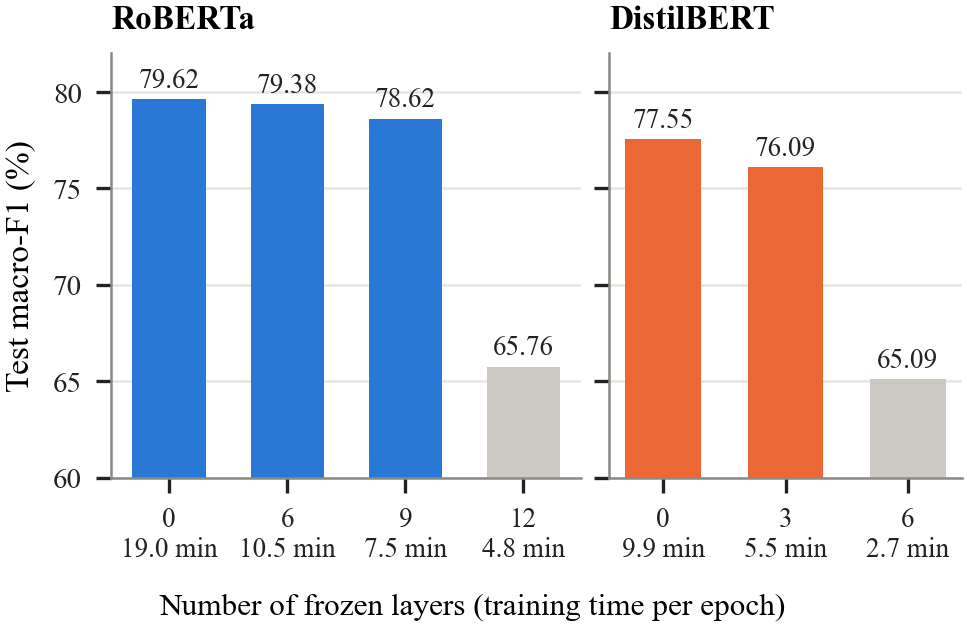
\includegraphics[width=\columnwidth]{fig_frozen_layers_en}
\caption{Test macro-F1 by number of frozen layers in early fusion. The numbers below the axis show the training time per epoch. Grey bars are fully frozen models (one seed); the other bars are means over three seeds.}
\label{fig:frozen}
\end{figure}

\subsection{Effect of the Parent Comment}
The Friedman test showed a difference in macro-F1 among the three inputs ($p = 0.009$, $W = 0.78$). As shown in Fig.~\ref{fig:input}, the parent increased macro-F1 for both models, by 1.10 and 0.69 points with early fusion and by 0.78 and 0.72 points with late fusion for RoBERTa and DistilBERT. All four gains were significant under the paired t-test and McNemar. The additional cost of early fusion was small: training time increased by only 1.15--1.16 times, batch-1 latency and memory barely changed, and only the per-example latency at batch size 32 roughly doubled.

\begin{figure}[t]
\centering
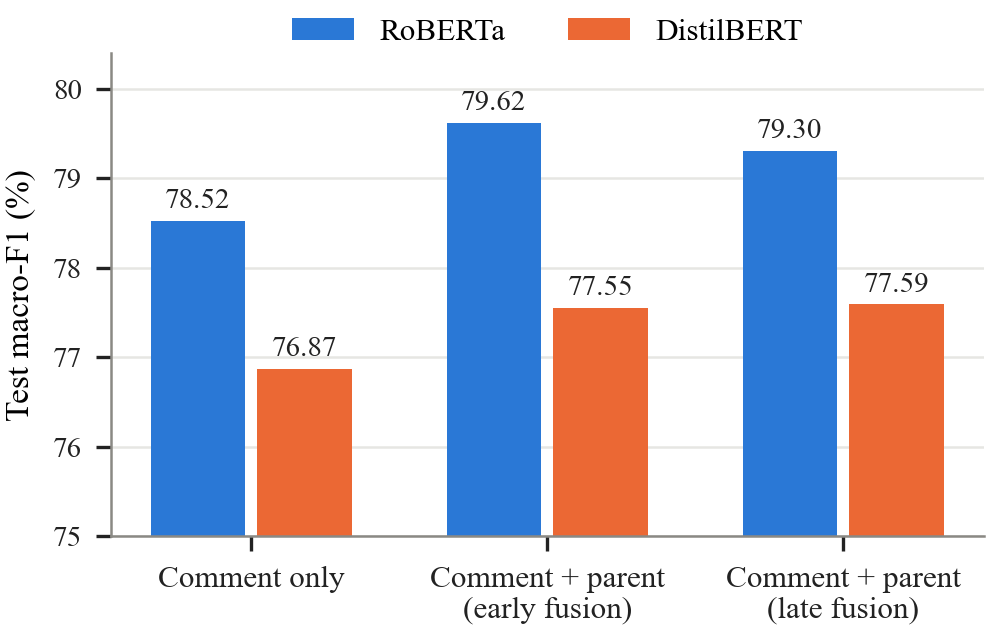
\includegraphics[width=\columnwidth]{fig_macro_f1_input_en}
\caption{Test macro-F1 for each model and input configuration (mean over three seeds). The vertical axis starts at 75\% so that differences between configurations are visible.}
\label{fig:input}
\end{figure}

The benefit of the parent was not uniform. On the 10,737 comments for which the RoBERTa comment-only model was uncertain, early fusion increased RoBERTa macro-F1 by 8.18 points, but only by 0.25 points on confidently predicted comments. The gain on comments of 1--3 words (2.59 points) was also larger than on comments longer than 10 words (0.71 points), and on the 5,886 comments (593 unique sentences) that appear with different labels the gain was 2.73 points. Even so, the parent corrected an average of 6,236 RoBERTa predictions per seed while turning 5,119 others wrong.

\subsection{Best Fusion Strategy}
For RoBERTa, early fusion outperformed late fusion by 0.32 points (95\% CI 0.15--0.49, $p_{\mathrm{Holm}} = 0.023$), which was also significant under McNemar. For DistilBERT, the two were equivalent (77.55\% and 77.59\%), and when pooled the advantage of early fusion was not significant ($p_{\mathrm{Holm}} = 0.158$). Late fusion was the most expensive configuration, with about 1.5 times the training time, 1.62--1.64 times the memory, and 1.70--1.79 times the batch-1 latency of early fusion.

\section{Discussion}

\subsection{Trade-off between RoBERTa and DistilBERT}
RoBERTa is more accurate, but only by 1.65--2.07 points at about twice the cost, so DistilBERT retains 97--98\% of the RoBERTa macro-F1 with roughly half the resources. This cost ratio is nearly the same for all three inputs, so it is most likely determined by model size. RoBERTa suits cases where accuracy is the priority, such as offline analysis, whereas DistilBERT suits cases with limited latency and memory, such as moderation tools that process comments continuously.

\subsection{Layer Freezing and Distillation}
The number of frozen layers affects performance, but not linearly. Freezing half of the RoBERTa layers reduced macro-F1 by only 0.24 points, while training time fell by 45\% and memory by 47\%, in line with \cite{ardakani2024slimfit}. A clear drop appeared only at 9 layers and became very large when all layers were frozen, so the pretrained representations still need fine-tuning. DistilBERT dropped faster, probably because it has fewer layers. Freezing saves only training cost and thus suits models that are retrained often, whereas DistilBERT saves inference cost.

\subsection{Role of the Parent Comment}
The parent improves the performance of both models, although only by about one point on average, because most comments can be understood from their own content. The parent matters when a comment is ambiguous, for example the reply ``;)'', which appears 68 times in the test data with only six sarcastic. As a reply to ``Sarcasm doesn't translate well through text. Haha'' it is sarcastic, but as a reply to ``What is your Guilty Pleasure?'' it is not, while a model without the parent must give the same prediction for both. This gain is much smaller than that reported by Dubey et al.\ (7.1 points \cite{dubey2026efficient} and 6.8 points \cite{dubey2025unpacking}), who used 7,370 samples without punctuation and capitalization, a condition that may make the model rely more on the parent.

\subsection{Early Fusion and Late Fusion}
Early fusion was chosen as the best strategy because it is more accurate for RoBERTa, equivalent for DistilBERT, and much cheaper. In early fusion, comment tokens can attend to specific words in the parent at every layer, whereas in late fusion both texts are first compressed into vectors. Since sarcasm often depends on specific phrases in the parent, late fusion is less advantageous, although it may be useful when one parent receives many replies.

\subsection{Comparison with Other Studies and Limitations}
The higher scores in \cite{dubey2026efficient} (F1 95.6\%) and \cite{zhang2025enhancing} (0.917) were obtained with different data sizes, preprocessing, and evaluation protocols, and none states whether the ``/s'' fragments (Section~\ref{sec:data}) were removed. The cost ratio, however, is consistent: the RoBERTa training time on SARC in \cite{dubey2026efficient} is 1.76 times that of DistilBERT (8.1 and 4.6 hours), compared with 1.92--1.94 times here.

This study has several limitations. First, training was limited to three epochs, even though 24 of the 29 final runs reached their best validation score at the last epoch. Second, only one dataset was used and its labels come from the ``/s'' marker, so sarcastic comments without the marker are recorded as non-sarcastic \cite{khodak2018sarc}. Third, the frozen models used the learning rate from full fine-tuning, the fully frozen models used only one seed, and each per-configuration test had only three pairs. Finally, large language models were not included and efficiency was measured on a single GPU.

\section{Conclusion}
RoBERTa is more accurate than DistilBERT for sarcasm detection on SARC, but its advantage is only about two macro-F1 points at roughly twice the computational cost. The number of frozen layers affects performance, but half of the RoBERTa layers can be frozen with a very small drop to save training cost. The parent comment improves the performance of both models, and early fusion is the best strategy because it is the most accurate for RoBERTa and cheaper than late fusion. RoBERTa with early fusion is recommended when accuracy is the priority, whereas DistilBERT with early fusion suits limited latency and memory. Future work could extend training, search for learning rates specific to frozen models, test other datasets, and compare with large language models.

\bibliographystyle{IEEEtran}
\bibliography{references}

\end{document}
